% -*-latex-*-
\documentclass[12pt,oneside]{mitthesis}
\usepackage{lgrind}
\usepackage{cmap}
\usepackage{natbib}
\usepackage{graphicx}
\usepackage{amsmath}
\usepackage{amssymb}
\usepackage{amsthm}
\usepackage{tikz}
\usetikzlibrary{shapes.geometric,arrows.meta,positioning,fit}
\newtheorem{definition}{Definition}[chapter]
% Override MIT's hardcoded institution name (defined inside mitthesis.cls)
\def\MIT{RMIT UNIVERSITY}
\def\Mit{RMIT University}
\providecommand{\doi}[1]{doi:~\texttt{\detokenize{#1}}}
\pagestyle{plain}
% Float layout: pack floats to the top of float-only pages instead of
% spreading them with blank space, and prefer mixing floats with text.
\makeatletter
\setlength{\@fptop}{0pt}
\setlength{\@fpsep}{12pt plus 4pt}
\setlength{\@fpbot}{0pt plus 1fil}
\makeatother
\renewcommand{\topfraction}{0.85}
\renewcommand{\bottomfraction}{0.6}
\renewcommand{\textfraction}{0.1}
\renewcommand{\floatpagefraction}{0.75}
\def\files{all}
\def\all{all}
\ifx\files\all \typeout{Including all files.} \else \typeout{Including only \files.} \includeonly{\files} \fi
\begin{document}
% -*-latex-*-
%
% Adapted from the MIT thesis template for RMIT University Vietnam submission.
% Course: COSC2993 - Minor Thesis/Project Part B
\title{\huge{Mitigating Evaluative Epistemic Filtering in LLM-Driven Essay Scoring: A Culturally-Aware Multi-Perspective Scoring (CAMPS) Framework}}
\author{Bao Nguyen}
\department{School of Science, Engineering and Technology}
\degree{Master of Artificial Intelligence}
\degreemonth{September}
\degreeyear{2026}
\thesisdate{September 2026}
% RMIT does not use MIT's copyright assignment. Thesis remains copyright to author.
\copyrightnoticetext{\copyright\ Bao Nguyen, 2026. All rights reserved.}
\supervisor{Dr Ginel Dorleon}{RMIT University}

% harmless placeholder text instead of leaving it blank.
\chairman{Dr Thuy Nguyen, Course Coordinator}{School of Science, Engineering and Technology}
\maketitle
\cleardoublepage
\setcounter{savepage}{\thepage}
%% RMIT requires a Declaration section (signed and dated).
\section*{Declaration}
I certify that except where due acknowledgement has been made, this thesis
is my own work, that any help received in preparing this thesis has been
acknowledged, and that all sources used have been indicated. I certify that
the work is original and has not been submitted previously, in whole or in
part, for any other academic award. Any use of generative AI tools in the
preparation of this thesis has been disclosed in accordance with course
policy.
\vspace{2cm}
\noindent Student name: Bao Nguyen \\
\noindent Student number: s4139514 \\
\noindent Signature: \dotfill \\
\noindent Date: \dotfill
\cleardoublepage
%% RMIT front-matter order (assessment specification): Title, Declaration,
%% Acknowledgements, Summary, Abstract, Contents.
\section*{Acknowledgements}
% -*-latex-*-
I would like to thank my supervisor, Dr Ginel Dorleon, for his guidance,
direction, and foundational work on multi-perspective bias mitigation
that inspired the CAMPS framework. I also thank Dr Thuy Nguyen, the
course coordinator, for her support throughout the semester, and RMIT
University Vietnam and the School of Science, Engineering and Technology
for the resources provided during this research.

\medskip
\noindent\textbf{Use of generative AI.} In accordance with course
policy, the use of generative AI tools in this project is disclosed
here. AI assistance (principally Claude, Anthropic) was used for
software engineering support in the experiment pipeline and analysis
scripts, for copy-editing and restructuring of prose drafted by the
author, for checking citations against primary sources, and for
examiner-style review of draft versions, whose comments the author
evaluated and acted on. The research
questions, framework design, experimental decisions, data collection,
interpretation of results, and conclusions are the author's own; no
experimental result was generated by an AI tool other than the LLM
evaluators that are the object of study, and every statistic is
regenerated by script from logged model outputs.

\cleardoublepage
%% RMIT requires a non-technical Summary (<200 words) for public dissemination.
\section*{Summary}
% -*-latex-*-
% Non-technical Summary, for a general audience. RMIT requirement: <200 words
% (counted as printed).

A Vietnamese student opens her essay with her grandfather's proverb,
``water wears down stone'', and argues as many Asian traditions
teach: context first, conclusion arrived at rather than announced. A
human examiner sees the skill. An AI grader trained mostly on Western
text may see only a missing thesis statement and mark her down for
the shape of her reasoning.

AI now grades high-stakes essays. This thesis measures that penalty
and proposes CAMPS: a panel of AI judges, each reading the essay
through a different cultural lens, disagreement flagging it for a
teacher.

Every AI model tested scored native-English essays above upper-level
Southeast Asian ones, the widest gap over a full band. Because no
human had judged the two groups to be of equal quality, this is a
disparity, not a proven cultural bias. The panel narrowed the gap by
about a quarter on the two most disparate models, widened it on one,
and more judges did not help; the disagreement signal proved too
coarse, and too loosely tied to cultural disagreement, to pick out
the essays needing a human. Any AI grader's gap can now be measured
before it is trusted; no single cultural lens should grade alone.

\cleardoublepage
\begin{abstractpage}
% -*-latex-*-
% RMIT requirement: technical abstract, <200 words (counted as printed).

Large language models (LLMs) increasingly score student essays, yet
models trained mainly on Western text risk treating Anglo-American
rhetoric as the standard and penalising other valid traditions. This thesis formalises the mechanism as \emph{evaluative
epistemic filtering} and develops CAMPS (Culturally-Aware
Multi-Perspective Scoring), an inference-time framework where
agents calibrated to distinct cultural readings of the rubric score
each essay independently, a Bias Divergence Score (BDS) measuring
disagreement. Across 200 topic-controlled
ICNALE essays and four model families, every baseline model scored
native-English above upper-band Southeast Asian writers
(0.19--1.18 bands; all 95\% intervals exclude zero). As the cohorts
were not matched on judged quality, this is an unadjusted disparity,
not an isolated cultural bias. A
three-agent panel reduced the disparity by 23--28\% on the two most
disparate models, by marking both cohorts down (natives more) and by no more than
its Southeast Asian lens alone; it amplified the disparity on the least disparate model. Five agents
added nothing on GPT-4o and widened the gap on Claude. Reweighting showed no trade-off with band association. BDS missed its detection target (held-out sensitivity 0.06 and
0.00 at 5\% false-positive rate). Culturally framed prompts change LLM scoring
in model-dependent ways; cohort gaps and agent disagreement are
imperfect fairness proxies.

\end{abstractpage}
%%%%%%%%%%%%%%%%%%%%%%%%%%%%%%%%%%%%%%%%%%%%%%%%%%%%%%%%%%%%%%%%%%%%%%

\pagestyle{plain}
  % -*- Mode:TeX -*-
%% This file simply contains the commands that actually generate the table of
%% contents and lists of figures and tables.  You can omit any or all of
%% these files by simply taking out the appropriate command.  For more
%% information on these files, see appendix C.3.3 of the LaTeX manual. 
\tableofcontents
\newpage
\listoffigures
\newpage
\listoftables

\newpage
\section*{Abbreviations}
\begin{tabular}{ll}
ASAP & Automated Student Assessment Prize (essay dataset) \\
AUC & Area Under the ROC Curve \\
AES & Automated Essay Scoring \\
AI & Artificial Intelligence \\
API & Application Programming Interface \\
BDS & Bias Divergence Score \\
CAMPS & Culturally-Aware Multi-Perspective Scoring \\
CEFR & Common European Framework of Reference for Languages \\
CI & Confidence Interval \\
CRI & Cultural Rubric Interpretation \\
ENS & English Native Speaker (ICNALE cohort) \\
FPR & False Positive Rate \\
GRA & Global Rating Archives (ICNALE module) \\
ICNALE & International Corpus Network of Asian Learners of English \\
IELTS & International English Language Testing System \\
L1 & First (native) language \\
LLM & Large Language Model \\
QWK & Quadratic Weighted Kappa \\
ROC & Receiver Operating Characteristic \\
SD & Standard Deviation \\
SEA & Southeast Asia(n) \\
TOEFL & Test of English as a Foreign Language \\
WE & Written Essays (ICNALE module) \\
WEIRD & Western, Educated, Industrialised, Rich, Democratic \\
WEP & Written Essays Plus (ICNALE module) \\
\end{tabular}

%% ------------------------------------------------------------
%% RMIT required structure (COSC2993):
%%   1. Introduction
%%   2. Literature Review
%%   3. Methods
%%   4. Results and Discussion
%%   5. Conclusion
%% ------------------------------------------------------------
\chapter{Introduction}
\label{chap:introduction}

\section{Problem Statement}
\label{sec:problem}

Automated Essay Scoring (AES) has entered a new era. Where earlier
systems counted surface features such as word length, sentence
complexity, and spelling, large language models (LLMs) now evaluate what previous
systems could not: the quality of a student's argument. Frontier models
are increasingly deployed to score high-stakes writing at scale,
promising consistent, rapid, and inexpensive assessment. Yet a model
that judges \emph{how well a student argues} must hold some standard of
what good argumentation looks like, and that standard is not neutral.
LLMs derive their evaluative expectations from training corpora that
overwhelmingly represent Western, Educated, Industrialised, Rich, and
Democratic (WEIRD) cultural contexts; empirical work has shown that
widely used models express cultural values closely aligned with
English-speaking and Protestant-European countries
\citep{tao2024cultural}.

Consider an illustration. A Vietnamese student opens an argumentative
essay with her grandfather's proverb, \emph{nuoc chay da mon} (water
wears down stone).
%% NOTE: proverb romanised deliberately -- mitthesis.cls under pdflatex
%% does not support Vietnamese diacritics without vntex/XeLaTeX.
She then develops her position the way many Asian
academic writing traditions teach: context first, evidence accumulated
gradually, the conclusion arrived at rather than announced. A trained
human examiner can recognise the coherence of this inductive structure.
An LLM evaluator calibrated by its training distribution to expect a
thesis statement in the opening paragraph may instead record ``lacks a
clear thesis'' and ``argument feels indirect''. It may also penalise the
hedging forms that signal politeness in her tradition as weak
reasoning. If so, she loses marks not because her English is poor, but
because the shape of her reasoning is culturally unfamiliar to the
model.

This thesis names this mechanism \emph{evaluative epistemic filtering}:
when an LLM evaluates writing, it applies an implicit cultural filter
derived from its training distribution, systematically discounting
rhetorical strategies that deviate from Anglo-American conventions
regardless of their argumentative merit. A pilot study in the preceding
phase of this research (Part~A) reported statistically significant
scoring disparities between Southeast Asian (SEA) and native-English
cohorts
of equivalent human-rated quality across two frontier models. The same
pilot reported that a culturally-diversified scoring panel reduced the
disparity. Those findings motivated, but do not yet establish, the
claims this thesis investigates at scale.

The problem this thesis addresses can therefore be stated plainly.
LLM-based essay scoring applies culturally partial standards,
invisibly and at scale, to students whose academic futures depend on
the result. The disparity is documented, but no validated framework
exists to mitigate it in evaluative settings. Nor does any calibrated
mechanism exist to detect the essays it affects. This thesis
quantifies the problem across models, builds and tests such a
framework, and tests its detection mechanism against human ground
truth.

\section{Research Questions and Hypotheses}
\label{sec:rqs}

Two research questions drive this thesis:

\begin{description}
  \item[RQ1.] To what extent does evaluative epistemic filtering
        manifest as measurable scoring disparities against Southeast
        Asian rhetorical patterns in LLM-driven essay scoring, and does
        it generalise across model families?
  \item[RQ2.] Can a culturally-aware multi-agent scoring architecture
        mitigate these disparities at inference time, without
        retraining or access to model weights, while reliably
        detecting the essays it cannot fairly score?
\end{description}

These questions are operationalised as four testable hypotheses:

\begin{itemize}
  \item \textbf{H1 (Generalisation).} Evaluative bias against Southeast
        Asian rhetorical patterns appears as a native$-$SEA cohort
        score gap whose 95\% confidence interval excludes zero on at
        least four LLMs, including an open-weight model.
  \item \textbf{H2 (Mitigation).} A five-agent culturally-calibrated
        panel with a meta-adjudicator reduces the cohort score gap
        more than the three-agent pilot configuration, without
        degrading agreement with the corpus's proficiency bands.
  \item \textbf{H3 (Detection).} A Bias Divergence Score threshold
        calibrated by receiver operating characteristic (ROC) analysis
        attains at least 90\% sensitivity at no more
        than a 5\% false-positive rate against multi-rater human
        disagreement on the 140-essay Global Rating Archives (GRA)
        validation set.
  \item \textbf{H4 (Trade-off boundary).} Consensus-weight allocation
        exhibits an identifiable boundary beyond which cohort-fairness
        gains degrade scoring accuracy against graded ground truth.
\end{itemize}

The research questions and hypotheses relate as follows. RQ1 is a
question about the \emph{existence and generality} of the problem; it
is operationalised by H1, which makes it falsifiable by fixing the
scope (four model families) and the test (statistical significance of
the cohort scoring gap). RQ2 is a question about the \emph{solution},
and it decomposes into three parts: whether the mitigation works (H2),
whether its failures can be detected (H3), and what the mitigation
costs (H4). Table~\ref{tab:rq-hypotheses} summarises the mapping and
where each hypothesis is tested.

\begin{table}[htbp]
\centering
\caption[Mapping of research questions to hypotheses]{How the research
questions decompose into hypotheses, and where each is tested.}
\label{tab:rq-hypotheses}
\small
\begin{tabular}{llll}
\hline
RQ & Hypothesis & Establishes & Tested in \\
\hline
RQ1 & H1 & Bias exists and generalises across models & Experiment E1 \\
RQ2 & H2 & The panel mitigates the bias & Experiments E1--E2 \\
RQ2 & H3 & Residual bias is detectable (BDS) & Experiment E3 \\
RQ2 & H4 & What mitigation costs in accuracy & Experiment E2 \\
\hline
\end{tabular}
\end{table}

Chapter~5 returns to each hypothesis explicitly. Because several
terms recur throughout, Table~\ref{tab:key-terms} defines them once
in plain language.

\begin{table}[htbp]
\centering
\caption[Key terms used in this thesis]{Key terms used in this
thesis, in plain language.}
\label{tab:key-terms}
\small
\begin{tabular}{p{3.3cm} p{8.9cm}}
\hline
Term & Meaning in this thesis \\
\hline
Evaluative epistemic filtering & The tendency of an AI grader to mark
down writing whose rhetorical form is unfamiliar from its training
data, regardless of the argument's quality. \\[2pt]
Lens & One AI evaluator given a documented cultural interpretation of
the same scoring rubric (Western, Southeast Asian, East Asian,
Mekong, or Neutral). \\[2pt]
Panel, consensus & Several lenses scoring the same essay
independently; their weighted average is the consensus score. \\[2pt]
Bias Divergence Score (BDS) & How much the lenses disagree on one
essay; high values are meant to flag the essay for a human. \\[2pt]
Cohort, cohort gap & A group of essays by writer background (Southeast
Asian learners or native-English writers); the gap is the difference
in mean score between the two cohorts. \\[2pt]
Band & The 1--9 integer score an evaluator assigns; the corpus's own
proficiency labels are CEFR bands (B1\_2, B2+). \\
\hline
\end{tabular}
\end{table}

\section{Theoretical Framing: Epistemic Injustice and Contrastive Rhetoric}
\label{sec:theory}

Two established bodies of theory ground this thesis. The first is
\citet{fricker2007epistemic}'s account of \emph{testimonial injustice}:
a speaker is wronged in their capacity as a knower when prejudice in
the hearer deflates the credibility of their testimony. Evaluative
epistemic filtering can be understood as testimonial injustice
automated and scaled: the student's argument is discounted not on its
merits but because its form does not match the evaluator's culturally
conditioned expectations. Fricker's framework also cautions against a
naive remedy: no evaluator, human or artificial, judges from nowhere.
This thesis therefore treats a ``culturally neutral'' evaluator as a
regulatory ideal rather than an achievable design goal, and pursues
\emph{plurality} of perspectives rather than pretended neutrality.

The second grounding is contrastive rhetoric. Since
\citet{kaplan1966cultural} first observed that rhetorical organisation
is culturally learned, research summarised by
\citet{connor2011intercultural} has documented systematic differences
between writing traditions. These include the distinction between
writer-responsible and reader-responsible coherence, and the validity of
inductive, context-first argument structures common in Asian academic
writing. This literature supplies the scholarly basis for the cultural
rubric interpretations at the centre of the proposed framework,
distinguishing them from ad-hoc cultural personas.

The mitigation strategy itself extends the formal multi-perspective
bias-reduction framework of \citet{dorleon2026uncovering}, who proved
that, under ideal conditions, generating text from multiple cultural
perspectives with bias filtering can eliminate stereotypical content
and perspective omission in \emph{generative} tasks. Companion
empirical work documented pervasive cultural bias in LLM treatments of
Southeast Asian content \citep{shujaa2026llms}. This
thesis asks whether those principles transfer from generation to
\emph{evaluation}. Independent support for the core mechanism comes
from the evaluation literature: panels of diverse LLM judges have been
shown to outperform and de-bias single large judges
\citep{verga2024replacing}, though with diversity defined by model
provider rather than by culture. The thesis, in short, tests whether
the jury effect holds when the axis of diversity is cultural.

Finally, the fairness--accuracy trade-off at the centre of H4 has a
direct lineage in fairness-aware machine learning.
\citet{dorleon2022feature} formulated feature selection as an explicit
trade-off between fairness and prediction performance. FAPFID
\citep{dorleon2023fapfid} then showed that fairness for unprivileged
groups can be improved without sacrificing overall performance,
through balanced representation. H4 asks whether an analogous frontier
exists in evaluative scoring, and where it lies.

\section{Significance}
\label{sec:significance}

The significance of this work is threefold. First, equity: as LLM-based
assessment becomes a gatekeeper to scholarships, university admission,
and migration pathways, a systematic penalty against non-Western
rhetorical traditions would constitute discrimination embedded in
infrastructure, invisible to its subjects and deniable by its
operators. Quantifying that penalty rigorously is a precondition for
governing it. Second, method: existing multi-agent AES research
improves accuracy without cultural awareness
\citep[e.g.,][]{su2025cafes}, while existing debiasing research targets
generative outputs rather than evaluative judgements; a validated
framework for \emph{evaluative} fairness would fill a documented gap at
their intersection. Third, deployability: because the proposed
framework operates entirely at inference time through commercial APIs,
any institution can apply it without retraining models. This practical
property distinguishes it from training-time approaches and
matches the constraints of real educational deployments, particularly
in the Southeast Asian context where this research is situated.

\section{Contributions}
\label{sec:contributions}


This thesis makes five contributions:

\begin{enumerate}
  \item \textbf{Conceptual:} it formalises evaluative epistemic
        filtering as a distinct bias mechanism in LLM-driven scoring,
        theoretically grounded in epistemic injustice and contrastive
        rhetoric.
  \item \textbf{Architectural:} it develops CAMPS (Culturally-Aware
        Multi-Perspective Scoring), a five-agent culturally-calibrated
        scoring panel with a meta-adjudicator, extending formal
        multi-perspective bias reduction from generation to evaluation.
  \item \textbf{Empirical:} it evaluates the framework on approximately
        200 topic-controlled essays from the ICNALE corpus
        \citep{ishikawa2023icnale} across four frontier and open-weight
        models, re-establishing the pilot evidence at scale on a corpus
        purpose-built for the comparison.
  \item \textbf{Methodological:} it introduces the Bias Divergence
        Score as a candidate trigger for targeted human review, and
        evaluates it against multi-rater human ground truth.
  \item \textbf{Practical:} it characterises the fairness--accuracy
        trade-off frontier, giving deploying institutions an explicit
        account of what fairness currently costs.
\end{enumerate}

\section{Thesis Outline}
\label{sec:outline}

The thesis follows the research questions in order. Chapter~2
reviews the literature that frames RQ1 and RQ2 and locates the gap
this thesis occupies. Chapter~3 develops the CAMPS framework and the
method: the data, the three experiments (E1 for H1 and part of H2,
E2 for H2 and H4, E3 for H3), the statistical protocol, and the alternatives
considered. Chapter~4 reports the experiments in that order and
discusses what the results mean, why they arose, how they compare
with prior work, and where they are uncertain. Chapter~5 answers each
hypothesis, states the contributions and limitations, and outlines
future work.
   % Introduction
\chapter{Literature Review}
\label{chap:literature}

The literature relevant to this thesis was searched between July and
September 2026 using Google Scholar, arXiv, the ACL Anthology, and the
Springer and IEEE digital libraries. The search combined the terms
``automated essay scoring'', ``multi-agent'', ``LLM-as-a-judge'',
``cultural bias'', ``debiasing'', ``fairness'', ``non-native writers'',
and ``contrastive rhetoric''. It was supplemented by backward and forward
citation chasing from key papers. Every reference cited in this thesis
was verified against its primary source. The review is organised
thematically: multi-agent and panel-based scoring
(Section~\ref{sec:lit-multiagent}), inference-time debiasing
(Section~\ref{sec:lit-debias}), cultural bias in LLMs
(Section~\ref{sec:lit-culture}), fairness in AES for non-native writers
(Section~\ref{sec:lit-aes-fairness}), and the contrastive-rhetoric
foundations (Section~\ref{sec:lit-rhetoric}), before
Section~\ref{sec:lit-gap} locates the gap this thesis addresses.

\section{Multi-Agent and Panel-Based Approaches to Scoring}
\label{sec:lit-multiagent}

Two research communities have converged on the same architectural
intuition, that several evaluators are better than one, for
different reasons.

In automated essay scoring, multi-agent designs pursue
\emph{accuracy}. CAFES \citep{su2025cafes} orchestrates scorer,
feedback-manager, and reflective-reviser agents (average 21\% QWK
improvement over direct prompting). Roundtable Essay Scoring
\citep[RES;][]{jang2025roundtable} consolidates trait-based evaluator
agents through simulated discussion (up to 34.86\% on ASAP,
zero-shot). Related designs add debate with retrieval
\citep{keramati2026madrag} and component recognition
\citep{wang2025autoscore}. What unites this family is the axis along
which agents differ: \emph{function} or \emph{trait}. None varies the
cultural interpretation of the rubric itself, and none evaluates
fairness across writer cohorts. Improvements are reported on
aggregate agreement. This leaves open the possibility that a more
accurate panel is uniformly accurate for some writers and uniformly
harsh for others.

In the LLM-evaluation community, panel designs pursue \emph{bias
reduction}. \citet{verga2024replacing} replaced a single large judge
model with a Panel of LLM evaluators (PoLL) drawn from three different
model families. They found that the panel not only correlated better
with human judgment across six datasets but also reduced intra-model
self-preference bias, at roughly a seventh of the cost. This is, to
date, the clearest empirical demonstration that judge \emph{diversity}
counteracts judge \emph{bias}. The diversity axis, however, is model
provider, chosen to decorrelate model-specific quirks rather than to
represent any substantive difference in evaluative standards. The
present thesis can be read as a targeted transplant. It takes the
panel-of-judges mechanism whose bias-reducing effect
\citet{verga2024replacing} established, and re-axes the diversity from
provider to \emph{cultural rubric interpretation}. Here the bias to be
countered is cultural rather than idiosyncratic.

\section{Inference-Time Debiasing}
\label{sec:lit-debias}

A second literature attacks bias at inference time, without retraining.
BiasFilter \citep{cheng2025biasfilter} periodically evaluates candidate
continuations during generation against a fairness reward model and
discards low-reward segments, enforcing fairness on \emph{generated
text} for both open-source and API-based models. The framework
demonstrates that meaningful debiasing is achievable purely at
inference time, a design constraint this thesis shares. But its
unit of intervention is the output token stream, which has no analogue
when the model's output is a single scalar score.

Closest to the present work is Multi-Agent Cultural Debate (MACD)
\citep{tan2026macd}, which assigns LLM agents explicit cultural
personas and orchestrates deliberation. MACD substantially raised the
rate of unbiased responses over single-model baselines, and its
central finding, that functionally-roled agent frameworks lack the
explicit cultural representation cross-cultural fairness needs,
independently corroborates the design principle behind CAMPS. The two
frameworks nonetheless answer different questions. MACD debiases
\emph{what a model says} in open-ended generation. CAMPS debiases
\emph{how a model judges}: the deliverable is a score whose
fairness can be measured cohort by cohort, and disagreement
between cultural agents is exploited as a detection signal rather than
dissolved through debate.

A caution for all multi-agent designs comes from the MALIBU benchmark
\citep{mirza2025malibu}, which shows that LLM-based multi-agent systems
can implicitly \emph{reinforce} social biases, and that
persona-conditioned judging can over-correct. For this thesis, MALIBU
motivates two design decisions: consensus weights are calibrated
empirically rather than assumed benign (Hypothesis H4 measures the
over-correction frontier directly), and panel behaviour is validated
against multi-rater human ground truth rather than taken on faith.
A separate line of work mitigates bias inside the model rather than
around it. Self-debiasing exploits a model's own ability to recognise
undesirable properties of its output, suppressing them at decoding
time \citep{schick2021self}, and FairSteer intervenes on hidden-layer
activations with dynamically applied steering vectors at inference
time \citep{li2025fairsteer}. Both are effective in their settings,
but both are white-box methods: they require access to output
distributions or internal activations that commercial scoring
deployments accessed through an API do not expose. CAMPS was
deliberately designed to operate at the level of prompts and outputs
alone, trading the precision of internal intervention for
applicability to any evaluator, including closed models.

\section{Cultural Bias in Large Language Models}
\label{sec:lit-culture}

That LLMs carry a Western-centric evaluative disposition is no longer
seriously contested. \citet{tao2024cultural} compared five OpenAI model
generations against nationally representative values-survey data for
107 countries. They found that model responses consistently resemble
those of English-speaking and Protestant-European populations. This is
the WEIRD alignment that this thesis takes as the distal cause of
evaluative epistemic filtering.

The proximal framework for this thesis comes from the supervisor's
research programme. \citet{dorleon2026uncovering} formally defined
bias categories for generative outputs (stereotyping, omission,
ethnocentrism, simplification) and proposed multi-perspective
generation with bias detection, proving that under ideal conditions the
method eliminates stereotypical content and perspective omission. The
companion study \citep{shujaa2026llms} evaluated seven state-of-the-art
LLMs on prompts embedding culturally sensitive assumptions about
Vietnam, Myanmar, and Nepal, documenting pervasive stereotyping,
linguistic ethnocentrism, and epistemic bias, with substantial
variation across models. It is this cross-model variation that
motivates testing H1 on at least four model families. The same group's work on
framing-bias detection \citep{shujaa2025framing} reflects the
detection-oriented strand of this programme that the Bias Divergence
Score continues: bias treated not only as something to remove but as
something to \emph{measure and flag}.
Two further studies shaped how cultural calibration is implemented in
this thesis. SEA-HELM, a community-built evaluation suite for
Southeast Asian languages, argues that benchmarks produced by machine
translation or synthetic generation without community input lose
cultural authenticity \citep{susanto2025seahelm}. The same reasoning
led this thesis to ground its cultural lenses in the contrastive
rhetoric literature and in a corpus built in the region, rather than
in ad hoc persona descriptions. More cautionary still,
\citet{khan2025randomness} showed that survey-based measures of LLM
cultural alignment are unstable across presentation formats and that
prompting a model to represent a specific culture is not reliably
steerable. For CAMPS this is a design constraint, not a refutation:
lens prompts are fixed verbatim (Appendix~A), decoding is
deterministic, and the panel's behaviour is validated empirically
against human raters (E3) rather than assumed correct because the
prompt requested it.

\section{Fairness in AES for Non-Native Writers}
\label{sec:lit-aes-fairness}

Concerns about equitable automated scoring of non-native writing
predate the LLM era. \citet{vajjala2018automated} showed on the
TOEFL11 and FCE corpora that the linguistic features most predictive of
essay quality differ across L1 populations, evidence that a single
scoring model implicitly encodes population-specific assumptions about
what good writing looks like. What has changed with LLM-based scoring
is the depth at which such assumptions operate: where feature-based
systems encoded them in engineered predictors that could be inspected,
LLM evaluators encode them in an opaque prior over rhetorical form
\citep[cf.][]{gallegos2024bias}.

The LLM-era evidence is accumulating quickly.
\citet{pack2024llm} evaluated four prominent LLMs (PaLM~2, Claude~2,
GPT-3.5, GPT-4) as scorers of English-learner placement essays,
finding usable reliability for the strongest model but meaningful
variation across models and administrations. Evaluative behaviour is
therefore model-specific, which motivates testing H1
across at least four model families rather than generalising from one.
Most directly relevant, \citet{gayed2026firstlanguage} fine-tuned an
open-weight model (Gemma-3-27B) for essay scoring and evaluated it on
the full TOEFL11 corpus of 12{,}100 essays across eleven L1
backgrounds, explicitly analysing scoring effects by first language.
The study documents L1-linked scoring variation on exactly the corpus
family and task that concern this thesis. Like the broader AES
fairness literature it extends, however, it stops at \emph{measurement}: no
mitigation framework is proposed, and the native/non-native design
this thesis requires is out of scope because TOEFL11 contains no
native-English cohort. Related recent work has begun to probe
mechanism as well as outcome. \citet{yang2025demographics} showed that
prompt-based LLM scorers can infer writer demographics, including
English-learner status, from essay text alone. They also showed that
scoring behaviour shifts once such a status is recognised.

Taken together, this literature establishes the disparity, its
model-dependence, and hints at its mechanism, while leaving the
mitigation side of the problem essentially untouched. That asymmetry
between diagnosis and treatment is the practical motivation for the
framework developed in Chapter~3.

\section{Contrastive Rhetoric and Cultural Writing Traditions}
\label{sec:lit-rhetoric}

The claim that rhetorical organisation is culturally learned, and
that an evaluator calibrated to one tradition will therefore
systematically misread another, has a research lineage of its own.
\citet{kaplan1966cultural} first argued that paragraph organisation
reflects culturally specific ``thought patterns'', contrasting the
linear development expected in English academic prose with the
patterns he observed in other traditions. The framework was refined
substantially in later work: \citet{hinds1987reader} distinguished
\emph{writer-responsible} languages, in which the burden of clarity
falls on the writer through explicit signposting, from
\emph{reader-responsible} languages, in which coherence is expected to
be inferred by the reader. Under this typology, the ``missing
thesis statement'' an LLM penalises may simply be reader-responsible
coherence operating as designed. \citet{connor2011intercultural}
consolidated this field as intercultural rhetoric, correcting early
essentialist readings: rhetorical traditions are conventions
distributed across writing communities, not fixed properties of
individuals. This thesis adopts that distinction explicitly, treating
L1 cohorts as proxies for rhetorical tradition rather than for
identity.

For Southeast Asian learner writing specifically, the empirical base
is anchored by the ICNALE project \citep{ishikawa2023icnale}, whose
topic-controlled design allows rhetorical variation to be observed
under matched task conditions across ten Asian countries and a
native-English reference cohort. This literature performs two duties in
the present thesis. First, it supplies the content of the cultural rubric
interpretations in Chapter~3, where each CRI prompt is grounded in
documented rhetorical conventions rather than improvised cultural
personas. Second, it supplies the defence against the objection that
culturally-calibrated agents merely role-play stereotypes. The
calibrations are drawn from a half-century of contrastive-rhetoric
scholarship, and their behaviour is tested empirically in Chapter~4.

\section{The Research Gap}
\label{sec:lit-gap}

Three literatures converge on the problem this thesis addresses, and
each stops short of it in a characteristic way. The multi-agent scoring
literature (Section~\ref{sec:lit-multiagent}) established that panels
of evaluators outperform single judges (CAFES and RES on accuracy,
PoLL on bias). But it defines panel diversity by function, trait, or
model provider, never by cultural interpretation of the rubric, and it
does not measure fairness across writer cohorts. The inference-time
debiasing literature (Section~\ref{sec:lit-debias}) established that
bias can be mitigated without retraining, and MACD specifically
established that \emph{explicit cultural representation} in agent
frameworks matters. But its object is generated text, not evaluative
judgment, and it dissolves inter-agent disagreement rather than
exploiting it. The cultural-bias literature
(Section~\ref{sec:lit-culture}) established the WEIRD disposition of
current models and, in \citet{dorleon2026uncovering}, provided a formal
multi-perspective mitigation framework with provable guarantees, for
generation only. Meanwhile, the AES fairness literature
(Section~\ref{sec:lit-aes-fairness}) continues to document L1-linked
scoring disparities without offering a validated mitigation framework.

The intersection itself remains empty: culturally-diverse rubric
interpretation, applied to evaluative scoring, with inter-agent
divergence used as a calibrated trigger for human review and validated
against multi-rater human ground truth. To the best of the searches
described above, no published work occupies it.
That intersection is precisely where CAMPS operates, and the recency of
the nearest neighbours on either side suggests the space will not
remain unoccupied for long.

\section*{Chapter summary}
Two literatures converge on the idea that several evaluators are
better than one, but neither varies the \emph{cultural} reading of
the rubric, and the fairness literature documents L1-linked scoring
disparities without a validated remedy. Chapter~3 builds the
framework that fills this gap and the experiments that test it.
   % Literature Review
\chapter{Methodology}
\label{chap:methodology}
% Target ~9 pages. Rubric criterion: "awareness and critical evaluation
% of alternatives" -- see Section 3.6.

\section{Working Theory: Evaluative Epistemic Filtering}
\label{sec:working-theory}

The framework developed in this chapter rests on a working theory of
why LLM evaluators systematically under-score culturally unfamiliar
writing. This section states that theory precisely, identifies the
conditions that sustain the phenomenon, and derives the observable
signatures that the experiments in Chapter~4 test.

\begin{definition}[Evaluative epistemic filtering]
\label{def:eef}
Let $E$ be an essay, $f_{\mathrm{human}}(E)$ the score assigned by a
trained human examiner under a rubric $R$, and
$f_{\mathrm{LLM}}(E \mid \theta)$ the score assigned by an LLM
evaluator whose parameters $\theta$ were estimated from a training
distribution $\mathcal{D}$. Evaluative epistemic filtering occurs when
\begin{equation}
\label{eq:eef}
\mathbb{E}\!\left[\, f_{\mathrm{LLM}}(E \mid \theta_{\mathcal{D}})
  - f_{\mathrm{human}}(E) \,\middle|\, c(E) \right] \neq 0,
\end{equation}
where $c(E)$ denotes the rhetorical tradition of the essay, and the
deviation is systematic in $c$: essays whose rhetorical form is
under-represented in $\mathcal{D}$ receive systematically deflated
scores relative to human judgment, independent of argumentative merit.
\end{definition}

The definition makes two commitments. First, the filter is a property
of the \emph{evaluator}, not of the essay: the same essay receives
different treatment under evaluators with different training
distributions. Second, the deviation is conditional on rhetorical
tradition rather than on language proficiency; this is what
distinguishes evaluative epistemic filtering from the legitimate
scoring of weaker English, and what the matched-cohort experimental
design in Section~\ref{sec:experimental-design} is built to isolate.

Four conditions jointly sustain the filter in current systems. First,
training corpora over-represent WEIRD cultural contexts, and models
demonstrably absorb the corresponding value orientation
\citep{tao2024cultural}. Second, the standards LLM evaluators apply
are opaque: unlike feature-based AES, where population-specific
predictors could be inspected directly \citep{vajjala2018automated},
an LLM's evaluative prior is distributed across its parameters
\citep{gallegos2024bias}. Third, diagnostic effort has concentrated on
generative outputs; the bias categories formalised by
\citet{dorleon2026uncovering} have no evaluative counterpart in the
literature. Fourth, the observable symptom (L1-linked scoring
disparities) is now documented \citep{gayed2026firstlanguage} but has
not been connected to a mitigation mechanism.

The theory yields three testable signatures, which map directly onto
the hypotheses of Chapter~1. First, a systematic scoring gap should
appear between rhetorical-tradition cohorts matched on human-rated
quality (H1). Second, the gap should shrink when the single evaluator
is replaced by a panel whose members embody different rubric
interpretations, because their individual filters are partially
decorrelated (H2). Third, panel members should disagree measurably on
precisely the essays where filtering operates, which makes divergence
itself a detection signal (H3).
The fairness--accuracy boundary (H4) follows from the consensus
mechanism and is derived in Section~\ref{sec:camps-framework}.

\section{The CAMPS Framework}
\label{sec:camps-framework}

CAMPS (Culturally-Aware Multi-Perspective Scoring) operationalises a
single design principle: if no evaluator judges from nowhere
(Section~\ref{sec:theory}), then fairness is pursued through a
\emph{plurality} of explicitly declared perspectives rather than
through a pretended neutrality. Concretely, the plurality is the panel
of five cultural rubric interpretations specified in
Section~\ref{sec:scaling-panel} (Western, Southeast Asian, East
Asian, Mekong/Vietnamese, and a neutral regulatory ideal; see
Table~\ref{tab:lens-panel}), each declared in an inspectable system
prompt rather than hidden in model weights, continuing the
multi-perspective principle introduced in
Section~\ref{sec:theory}. The framework operates entirely at
inference time, requires no model retraining or weight access, and
treats every underlying LLM as a black box reachable through an API.
Figure~\ref{fig:camps-architecture} shows the pipeline; the five
components are specified below.

\begin{figure}[htbp]
\centering
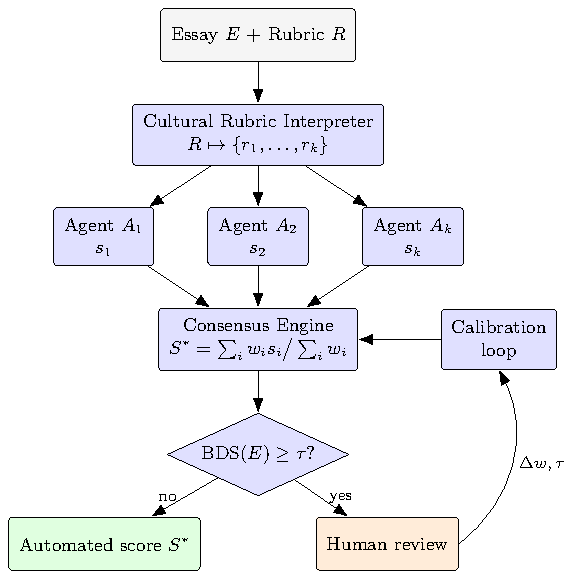
\includegraphics[width=0.72\textwidth]{figures/fig-camps-architecture}
\caption[The CAMPS pipeline]{The CAMPS pipeline. Each essay is scored
in parallel by $k$ \emph{culturally-calibrated} agents: LLM evaluators
whose system prompts embed a documented cultural interpretation of the
scoring rubric (Component~1). The consensus engine aggregates the
scores. The Bias Divergence Score routes contested essays to human
review, whose outcomes feed the calibration loop. CAMPS components are
shaded blue; inputs and outcomes are unshaded.}
\label{fig:camps-architecture}
\end{figure}

\subsection*{Component 1: Cultural Rubric Interpreter (CRI)}
Given the scoring rubric $R$, the CRI produces $k$ culturally-adapted
interpretations $\{r_1, \dots, r_k\}$ through system-level prompting.
Each interpretation is grounded in the contrastive-rhetoric literature
reviewed in Section~\ref{sec:lit-rhetoric} rather than in improvised
personas. The Southeast Asian interpretation, for example, instructs
the agent to recognise inductive thesis development and
reader-responsible coherence \citep{hinds1987reader} as valid
realisations of the rubric's coherence criterion. The neutral
interpretation is retained as a regulatory ideal in Fricker's sense
\citep{fricker2007epistemic}, not as an achievable standpoint.
The full prompt texts are reproduced verbatim in
Appendix~\ref{chap:appendix-prompts}.

\subsection*{Component 2: Evaluator agent pool}
Each interpretation is bound to an independent evaluator agent, and
each agent scores the essay without access to the other agents'
outputs:
\begin{equation}
s_i = A_i(E, r_i), \qquad i = 1, \dots, k,
\end{equation}
with temperature fixed at $t = 0.0$ and structured (JSON) output, so
that every run is deterministic and reproducible. Independence at this
stage is deliberate: the MALIBU results \citep{mirza2025malibu} caution
that interacting agents can amplify rather than cancel bias, so CAMPS
confines interaction to the aggregation stage, where it is
mathematically controlled.

\subsection*{Component 3: Consensus aggregation}
The panel's scores are combined as a weighted mean,
\begin{equation}
\label{eq:consensus}
S^{*}(E) = \frac{\sum_{i=1}^{k} w_i\, s_i(E)}{\sum_{i=1}^{k} w_i},
\qquad w_i \geq 0,
\end{equation}
with weights initialised equal. Because $S^{*}$ is linear in the
agents' scores, any reweighting that raises the expected score of one
cohort must lower another's whenever the agents disagree
systematically; this is the mechanism behind the fairness--accuracy
boundary hypothesised in H4, and Section~\ref{sec:experimental-design}
describes how the weight space is swept to locate it empirically.

\subsection*{Component 4: Bias Divergence Score (BDS)}
The framework's detection signal is the dispersion of the panel:
\begin{equation}
\label{eq:bds}
\mathrm{BDS}(E) = \sqrt{\frac{1}{k} \sum_{i=1}^{k}
  \bigl(s_i(E) - S^{*}(E)\bigr)^{2}}.
\end{equation}
A low BDS means the cultural interpretations converge: the essay is
scored the same way regardless of the lens, and the automated score can
be trusted. A high BDS means the lenses disagree, which under the
working theory is exactly the signature of an essay whose score depends
on culturally contingent expectations; such essays are flagged for
human review. The pilot fixed the threshold at $\tau = 0.75$ on the
operational argument that 0.75 standard deviations corresponds to a
two-band disagreement under IELTS-style scoring. Part~B replaces this
hand-set value with a threshold calibrated by receiver operating
characteristic analysis against multi-rater human ground truth (H3),
as specified in Section~\ref{sec:experimental-design}.

\subsection*{Component 5: Calibration loop}
Outcomes of human review feed back into the framework in two ways: the
consensus weights $w_i$ are re-optimised to maximise agreement with
human scores subject to a cohort-fairness constraint, and the
threshold $\tau$ is re-estimated as review outcomes accumulate. The
loop closes the system without touching model weights; everything
learned lives in $w$ and $\tau$.

\medskip
The five components divide the framework's labour: the first two
create and apply the plurality of perspectives, the third converts
plurality into a single defensible score, and the last two turn
residual disagreement into detection and adaptation. No component
alone mitigates the filter; the fairness properties of CAMPS are a
property of the assembly.
Table~\ref{tab:framework-comparison} positions CAMPS against the
frameworks reviewed in Chapter~2 along the five capabilities the
design combines.

\begin{table}[htbp]
\centering
\caption[Capability comparison of related frameworks]{Capability
comparison. \emph{Inf.} = inference-time only; \emph{Cult.} = explicit
cultural perspectives; \emph{Eval.} = evaluative (scoring) task;
\emph{Div.} = divergence-based detection; \emph{HITL} = calibrated
human-in-the-loop trigger.}
\label{tab:framework-comparison}
\begin{tabular}{lccccc}
\hline
Framework & Inf. & Cult. & Eval. & Div. & HITL \\
\hline
CultureLLM \citep{li2024culturellm} & $\times$ & \checkmark & $\times$ & $\times$ & $\times$ \\
BiasFilter \citep{cheng2025biasfilter} & \checkmark & $\times$ & $\times$ & $\times$ & $\times$ \\
CAFES \citep{su2025cafes} & \checkmark & $\times$ & \checkmark & $\times$ & $\times$ \\
RES \citep{jang2025roundtable} & \checkmark & $\times$ & \checkmark & $\times$ & $\times$ \\
PoLL \citep{verga2024replacing} & \checkmark & $\times$ & \checkmark & $\times$ & $\times$ \\
MACD \citep{tan2026macd} & \checkmark & \checkmark & $\times$ & $\times$ & $\times$ \\
Dorleon \& Shujaa \citeyearpar{dorleon2026uncovering} & \checkmark & \checkmark & $\times$ & $\times$ & $\times$ \\
\textbf{CAMPS (this thesis)} & \checkmark & \checkmark & \checkmark & \checkmark & \checkmark \\
\hline
\end{tabular}
\end{table}

Relative to the Part~A pilot, the framework specified here differs in
three respects, each developed in the following sections: the panel is
scaled from three to five cultural interpretations with a
meta-adjudicator (Section~\ref{sec:scaling-panel}), the corpus and
cohort design are rebuilt on data that supports the comparison
(Section~\ref{sec:data}), and both the consensus weights and the BDS
threshold are calibrated empirically rather than hand-set
(Section~\ref{sec:experimental-design}).

\section{Scaling the Panel: from Three to Five Agents}
\label{sec:scaling-panel}

The pilot panel comprised three rubric interpretations: Western,
Southeast Asian, and a neutral interpretation retained as a regulatory
ideal (Section~\ref{sec:camps-framework}). Scaling to five requires a
principled answer to the question \emph{which} cultural lenses to add.
Three selection criteria are applied. A candidate lens must be
(i)~\emph{documented}: its rhetorical conventions must be described in
the contrastive-rhetoric literature, so that the CRI prompt encodes
scholarship rather than stereotype; (ii)~\emph{validatable}: the
corpus must contain a writer cohort from the corresponding tradition,
so that the lens's behaviour can be checked against real essays; and
(iii)~\emph{distinct}: the lens must be expected to diverge from the
existing panel on identifiable essay features, otherwise it adds cost
without information.

Applying these criteria to the available data
(Section~\ref{sec:data}) selects an \emph{East Asian} lens, grounded
in the reader-responsible coherence tradition documented for Japanese
and related academic writing cultures \citep{hinds1987reader} and
validatable against ICNALE's China, Japan, Korea, and Taiwan cohorts,
and a \emph{Mekong/Vietnamese} lens, motivated by the region this
research serves and validatable against the ICNALE~WEP cohorts from
Vietnam, Cambodia, Laos, and Myanmar. A Middle Eastern lens, although
well documented in the contrastive-rhetoric literature, fails the
validatable criterion for the primary corpus and is deferred to future
work. Table~\ref{tab:lens-panel} summarises the resulting panel.

\begin{table}[htbp]
\centering
\caption[The five-lens CAMPS panel]{The five-lens panel: rhetorical
grounding and the corpus cohort against which each lens's behaviour
can be validated.}
\label{tab:lens-panel}
\small
\begin{tabular}{p{2.9cm} p{5.6cm} p{3.6cm}}
\hline
Lens & Rhetorical grounding & Validating cohort \\
\hline
CRI\textsubscript{Western} & Writer-responsible coherence; explicit
thesis-first linear development \citep{kaplan1966cultural,
connor2011intercultural} & ICNALE ENS \\[3pt]
CRI\textsubscript{SEA} & Inductive, context-first development;
collectivist framing \citep{connor2011intercultural,
ishikawa2023icnale} & ICNALE THA, IDN, PHL \\[3pt]
CRI\textsubscript{EastAsian} & Reader-responsible coherence; delayed
thesis; \emph{ki-sho-ten-ketsu}-style organisation
\citep{hinds1987reader} & ICNALE CHN, JPN, KOR, TWN \\[3pt]
CRI\textsubscript{Mekong} & Proverb- and narrative-anchored
argumentation observed in Mekong-region learner writing
\citep{ishikawa2023icnale, shujaa2026llms} & ICNALE WEP VNM, KHM,
LAO, MMR \\[3pt]
CRI\textsubscript{Neutral} & Regulatory ideal: argumentative merit
irrespective of structural ordering \citep{fricker2007epistemic} &
(all cohorts) \\
\hline
\end{tabular}
\end{table}

The second architectural addition is a \emph{meta-adjudicator}: a
further LLM instance that receives the five agents' scores and their
short written rationales, and produces a reasoned consensus score,
\begin{equation}
S^{\mathrm{adj}}(E) = M\bigl(s_1, \rho_1, \dots, s_k, \rho_k\bigr),
\end{equation}
where $\rho_i$ is agent $i$'s rationale. The adjudicator is blind to the writer's identity and cohort
metadata, and runs at $t = 0.0$ like the agents. It constitutes an
alternative aggregation path to the weighted mean of
Equation~\ref{eq:consensus}. Where the weighted mean treats every
agent's judgment as exchangeable evidence, the adjudicator can weigh
\emph{arguments}, for example discounting an agent whose rationale
misidentifies the essay's structure. Experiment
E2 compares the two paths directly, and the BDS of
Equation~\ref{eq:bds} is computed from the raw agent scores in both
conditions, so the detection signal is unaffected by the choice of
aggregator. This design responds to the caution from multi-agent bias
research \citep{mirza2025malibu}: the adjudicator adds deliberation
\emph{after} independent judgment, rather than allowing agents to
influence one another during scoring.

\section{Data}
\label{sec:data}

\subsection*{Corpus selection}
The experimental design requires a corpus with four properties: essays
by Southeast Asian learners identified by first language or country;
a native-English reference cohort writing under identical task
conditions; a human-assigned quality or proficiency measure; and terms
of use permitting research at this scale. A systematic search of the
major public learner corpora found exactly one corpus satisfying all
four. TOEFL11 \citep{blanchard2013toefl11}, used in the pilot phase,
contains 12{,}100 essays across eleven first languages but includes
no Southeast Asian L1 and, by construction, no native-English cohort,
and its proficiency labels are coarse (low, medium, high). ICLE~v3
covers twenty-five L1 backgrounds without Thai or another Southeast
Asian L1; ELLIPSE offers approximately 9{,}000 human-scored learner
essays without L1 labels; EFCAMDAT records nationality and CEFR level
but has no native reference cohort.\footnote{Corpus contents verified
against their official distribution pages in July 2026: TOEFL11 via
the Linguistic Data Consortium (LDC2014T06), ICLE via UCLouvain,
ELLIPSE via its public repository, EFCAMDAT via the EF--Cambridge
Open Language Database.} The ICNALE corpus family
\citep{ishikawa2023icnale} satisfies all four properties and is
therefore adopted.

\subsection*{The ICNALE corpus family}
ICNALE (the International Corpus Network of Asian Learners of
English) collects topic-controlled English essays and speeches from
college students across ten Asian countries and regions together with
a native-English-speaker reference cohort writing under identical
conditions. Three modules are used in this thesis
(Table~\ref{tab:icnale-modules}). Critically for the present design,
every written essay addresses the same two prompts (whether college
students should hold a part-time job, and whether smoking should be
banned in restaurants), under controlled length and time conditions;
this removes the prompt-variation confound present in TOEFL11's
eight-topic design. All learner participants are placed into
CEFR-linked proficiency bands (A2, B1\_1, B1\_2, B2+) on the basis of
standardised test scores or a vocabulary-size test, which enables
proficiency-matched cohort construction.

\begin{table}[htbp]
\centering
\caption[ICNALE modules used in this thesis]{ICNALE modules used in
this thesis (contents as published on the official ICNALE
distribution site, March 2026).}
\label{tab:icnale-modules}
\small
\begin{tabular}{p{3.2cm} p{4.6cm} p{4.6cm}}
\hline
Module & Contents & Role in this thesis \\
\hline
Written Essays (WE) v2.6 & 5{,}600 essays, 200--300 words, two
controlled topics; ten Asian countries/regions plus native ENS cohort
& Primary cohorts: SEA learners and native reference \\[3pt]
Written Essays Plus (WEP) v0.7 & 2{,}340 essays from additional
countries including Vietnam, Cambodia, Laos, Myanmar & Mekong cohort;
validation of CRI\textsubscript{Mekong} \\[3pt]
Global Rating Archives (GRA) v2.1 & 140 essays, each rated by 80
raters of varied L1 and occupational backgrounds (22{,}400 ratings)
& Multi-rater human ground truth for BDS validation (E3) \\
\hline
\end{tabular}
\end{table}

\subsection*{Cohort construction and sampling}
Figure~\ref{fig:sampling-flow} summarises the construction of the
experimental sample. The Southeast Asian cohort draws essays from the
Thailand, Indonesia, and Philippines components of the WE module,
optionally extended with the Vietnam component of WEP; the native
cohort draws from the ENS component. Both cohorts are restricted to
the two upper proficiency bands (B1\_2 and B2+) and stratified by
topic and band, with $n \approx 100$ essays per cohort drawn under a
fixed random seed. Restricting to the upper bands serves the same
purpose as the pilot's matched-score design: it narrows the range of
underlying proficiency so that systematic scoring differences between
cohorts cannot be attributed to proficiency alone, with residual
band-composition differences controlled in analysis. The GRA's 140
essays are retained in full as the validation set for Experiment E3,
since each carries eighty independent human ratings; inter-rater
dispersion in the GRA additionally provides a human benchmark against
which BDS values can be compared, essay by essay.

\begin{figure}[htbp]
\centering
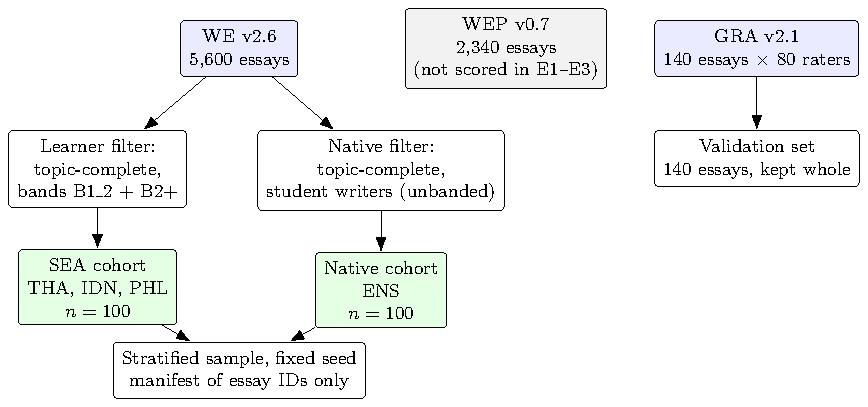
\includegraphics[width=0.8\textwidth]{figures/fig-sampling-flow}
\caption[Cohort construction and sampling flow]{Cohort construction
and sampling. Essay texts remain within licensed storage; the
reproducibility manifest records essay identifiers only.}
\label{fig:sampling-flow}
\end{figure}

\subsection*{Scoring target and ground truth}
Agents score each essay on the rubric's band scale; agreement with
ground truth is computed against the corpus's proficiency bands for
the main cohorts and against the GRA's multi-rater consensus for the
validation set. Inspection of the downloaded GRA archive (v2.1)
confirms its structure: each of the 140 essays carries ratings from
80 raters of varied L1 backgrounds, each scoring ten analytic
dimensions (0--10) grouped as Language, Content, and Attitude, plus a
holistic score out of 100. Per-essay rating dispersion across the 80
raters provides the human-disagreement benchmark against which BDS is
compared. Two properties of the archive shape the E3 design. First,
all 140 rated essays address the part-time-job prompt, so the
validation set is single-topic. Second, the raters disagree
substantially among themselves (mean within-essay standard deviation
of the Content ratings $\approx 1.8$ on the 0--10 scale):
disagreement among evaluators, human or artificial, is the normal
condition of essay assessment, and the question E3 asks is whether
the panel's divergence tracks the essays on which \emph{humans}
diverge.

\subsection*{Licence and handling}
ICNALE is distributed free for research; its terms of use prohibit
redistribution of any part of the data, and the project's required
citation is the ICNALE Guide \citep{ishikawa2023icnale}. In this
project, essay texts are stored only in access-controlled university
storage, never committed to version control, and no essay text is
reproduced in this thesis beyond short quotation where the licence
permits; the reproducibility package releases code, prompts,
configurations, and essay-ID manifests only. The data are
de-identified by the distributor, and their use falls under the
ethics exemption described in Section~\ref{sec:ethics}.

\section{Experimental Design}
\label{sec:experimental-design}

Three experiments test the four hypotheses
(Table~\ref{tab:experiments}). All conditions share the same
determinism guarantees: temperature fixed at $0.0$, structured JSON
outputs, exact model versions pinned in the experiment configuration,
and a fixed random seed for all sampling, so that every result in
Chapter~4 is reproducible from the released configuration, prompts,
and essay-identifier manifest.

\begin{table}[htbp]
\centering
\caption[Overview of Experiments E1--E3]{Overview of the three
experiments: data, conditions, and the hypotheses each tests.}
\label{tab:experiments}
\small
\begin{tabular}{p{1.2cm} p{3.4cm} p{4.3cm} p{2.2cm}}
\hline
Exp. & Data & Conditions & Tests \\
\hline
E1 & SEA + native cohorts ($n \approx 100$ each) & Single-agent
baseline vs.\ CAMPS $k{=}3$, four models & H1; H2 (part) \\[3pt]
E2 & Same cohorts & CAMPS $k{=}5$ with and without meta-adjudicator;
consensus-weight sweep ($\Delta w = 0.05$); ablation over
$k \in \{1,3,5\}$ & H2; H4 \\[3pt]
E3 & GRA validation set (140 essays $\times$ 80 raters) & CAMPS
$k{=}5$; ROC calibration of $\tau$ on a calibration split, evaluation
on a hold-out split & H3 \\
\hline
\end{tabular}
\end{table}

\textbf{Experiment E1 (scaled replication)} scores both cohorts under
the single-agent baseline and the pilot's three-agent panel on all
four models, establishing whether the gap exists at scale (H1) and
providing the $k{=}3$ reference for E2.

\textbf{Experiment E2 (extended architecture)} scores the same essays
under the five-agent panel, with and without the meta-adjudicator,
and sweeps the consensus weights in steps of $0.05$ under
$\sum_i w_i = 1$, tracing the fairness--accuracy frontier from which
H4's boundary is read off empirically. The ablation over $k$
separates the contribution of panel size from that of the
adjudicator.

\textbf{Experiment E3 (detection validation)} computes BDS for the
140 GRA essays. Human rating dispersion provides the reference notion
of a genuinely contested essay; the threshold $\tau$ is calibrated on
a random half of the GRA set (Youden's $J$) and evaluated on the
held-out half, reporting sensitivity, false-positive rate, and area
under the ROC curve.

\section{Alternatives Considered}
\label{sec:alternatives}

The rubric of this thesis requires critical awareness of alternatives;
this section records the designs considered and rejected, and why.

\emph{Training-time cultural adaptation}, as in CultureLLM
\citep{li2024culturellm}, fine-tunes models on culturally augmented
data. It is rejected on deployment grounds: it requires weight access
or fine-tuning budgets unavailable to most educational institutions,
must be repeated for every model generation, and cannot be audited by
the deploying institution. \emph{Activation steering}, as in FairSteer
\citep{li2025fairsteer}, intervenes on internal representations and is
infeasible for API-only access by construction
(Section~\ref{sec:lit-debias}).

\emph{Single-prompt debiasing}, instructing one evaluator to ``score
fairly across cultures'', was considered and rejected for two reasons:
it collapses the plurality of standards back into a single opaque
judgment, so cultural bias cannot be measured, only asserted away; and
it provides no divergence signal, so there is nothing to calibrate a
human-review trigger against. The single-agent baseline in E1
approximates this design and provides its empirical comparison.

\emph{Inter-agent debate}, as in MACD \citep{tan2026macd}, lets agents
deliberate before judgment. For evaluative scoring this is rejected on
two grounds: the MALIBU results \citep{mirza2025malibu} show that
agent interaction can amplify bias, and deliberation before scoring
destroys the independence that makes the Bias Divergence Score
meaningful. CAMPS instead confines deliberation to the optional
meta-adjudicator, which operates after independent scores are
recorded.

\emph{Recruiting external human raters} for validation was rejected on
ethics-scope and timeline grounds (Section~\ref{sec:ethics}); the GRA
archive supplies eighty raters per essay without new data collection.
Alternative corpora were considered and eliminated on design grounds
in Section~\ref{sec:data}.

\section{Ethical Considerations}
\label{sec:ethics}

This research analyses de-identified secondary data only and is
covered by an RMIT human research ethics exemption (Project ID 31036).
The ICNALE corpus is distributed for research with all personal
identifiers removed by the distributor; no attempt is made to
re-identify any writer, no essay text is redistributed or committed to
version control, and storage follows the project's research data
management plan (university-managed storage, access restricted to the
research team). Validation re-scoring is performed by the research
team only; no external participants are recruited, and any future
extension involving human participants would require a new ethics
assessment before commencing.

Two further considerations shape the design rather than merely
constrain it. First, cultural essentialism: scoring agents are
calibrated to \emph{documented rhetorical traditions}, not to
nationalities, and L1 cohorts are treated throughout as proxies for
rhetorical tradition rather than identity
(Section~\ref{sec:lit-rhetoric}). Second, downstream welfare: CAMPS is
designed as a human-in-the-loop system precisely because the cost of a
misclassified essay falls on a student; the BDS mechanism exists to
route uncertain judgments to a human rather than automate them. The
use of generative AI tools in this project is disclosed in accordance
with course policy.

\section{Metrics and Statistical Protocol}
\label{sec:metrics}

\textbf{Primary metric.} The primary fairness quantity is the
\emph{cohort score gap}: the difference in mean panel score between
the native and Southeast Asian cohorts,
\begin{equation}
\Delta = \overline{S^{*}}_{\mathrm{native}}
        - \overline{S^{*}}_{\mathrm{SEA}},
\end{equation}
computed on proficiency-matched cohorts so that, absent bias, the
expected gap is near zero. This operationalisation follows the pilot
and is forced by a property of the reference data: the native cohort
writes as an unbanded reference group (ICNALE assigns CEFR bands to
learners only), so band-agreement statistics are undefined for it.
Agreement with graded ground truth is reported secondarily where such
truth exists: Quadratic Weighted Kappa,
\begin{equation}
\kappa_w = 1 - \frac{\sum_{i,j} w_{ij} O_{ij}}
                     {\sum_{i,j} w_{ij} E_{ij}},
\qquad w_{ij} = \frac{(i-j)^2}{(R-1)^2},
\end{equation}
against proficiency bands for the learner cohorts, and against the
multi-rater human consensus for the GRA validation set (E3).

\textbf{Uncertainty.} Every reported statistic carries its $n$, and
every proportion or $\kappa_w$ is reported with a 95\% percentile
bootstrap confidence interval (10{,}000 resamples, fixed seed).
Following the statistical-reporting guidance adopted for this thesis,
confidence intervals are the primary inferential device;
$p$-values are reported only for the pre-registered hypothesis tests
(Fisher's $z$ on cohort correlation differences for H1), and no
post-hoc significance testing is performed on exploratory findings.

\textbf{Detection metrics.} BDS performance in E3 is reported as
sensitivity, false-positive rate, and area under the ROC curve on the
held-out split, with the calibrated threshold $\tau$ stated
explicitly.

\textbf{Weight calibration.} The E2 weight sweep reports the full
frontier rather than a single optimum: at each weight vector, the
cohort score gap (fairness) and $\kappa_w$ against CEFR bands on the
banded learner cohort (accuracy; the native reference is unbanded)
are recorded, and the H4 boundary is read off the resulting Pareto
frontier.

\textbf{Reproducibility.} All tables and figures in Chapter~4 are
generated by the analysis scripts in the project repository from the
logged scoring calls; no statistic is computed by hand. The
configuration file, prompts, essay-identifier manifest, and analysis
code are released; essay texts are not (Section~\ref{sec:data}).
   % Methods
\chapter{Results and Discussion}
\label{chap:results}
% Target ~12 pages -- the 40-point rubric criterion. All tables and
% figures generated by scripts for reproducibility. Include
% uncertainty/error analysis explicitly.

\section{Experiment 1: Evaluative Bias at Scale (H1)}
% Prose written after E1 completes; table auto-generated by
% Code/src/make_tables.py from the experiment logs.
Table~\ref{tab:e1-qwk} reports agreement with ground truth per model,
condition, and cohort.
%% TODO: results prose after E1.
Lorem ipsum dolor sit amet, consectetur adipiscing elit.

% AUTO-GENERATED by make_tables.py -- do not edit by hand.
\begin{table}[htbp]
\centering
\caption[E1: cohort score gap by model]{Experiment E1: mean consensus
score by cohort and the native$-$SEA score gap on proficiency-matched
cohorts, with 95\% bootstrap confidence intervals (10{,}000
resamples).}
\label{tab:e1-qwk}
\small
\begin{tabular}{llccc}
\hline
Model & Condition & Mean score\textsubscript{SEA} &
Mean score\textsubscript{native} & Gap [95\% CI] \\
\hline
Claude Sonnet & Baseline & 4.44 ($n$=100) & 5.62 ($n$=100) & 1.18 [0.86, 1.50] \\
Gemini Pro & Baseline & 4.83 ($n$=100) & 5.00 ($n$=17) & 0.17 [-0.14, 0.49] \\
GPT-4o & Baseline & 5.03 ($n$=100) & 5.83 ($n$=100) & 0.80 [0.60, 1.00] \\
GPT-4o & CAMPS $k{=}3$ & 4.70 ($n$=100) & 5.27 ($n$=100) & 0.57 [0.37, 0.78] \\
\hline
\end{tabular}
\end{table}


\section{Experiment 2: Extended CAMPS Panel (H2, H4)}
Table~\ref{tab:e2-ablation} reports the ablation over panel size and
the meta-adjudicator; the weight-sweep frontier is reported as a
figure generated from the same logs.
%% TODO: results prose after E2.
Lorem ipsum dolor sit amet, consectetur adipiscing elit.

% PLACEHOLDER -- overwritten by make_tables.py after E2 runs.
\begin{table}[htbp]
\centering
\caption[E2: ablation over panel size and adjudicator]{Experiment E2:
ablation over panel size $k$ and the meta-adjudicator. Values pending
completion of E2.}
\label{tab:e2-ablation}
\small
\begin{tabular}{lccc}
\hline
Configuration & QWK\textsubscript{SEA} & QWK\textsubscript{native} & Gap \\
\hline
Baseline ($k{=}1$) & -- & -- & -- \\
CAMPS $k{=}3$ & -- & -- & -- \\
CAMPS $k{=}5$ & -- & -- & -- \\
CAMPS $k{=}5$ + adjudicator & -- & -- & -- \\
\hline
\end{tabular}
\end{table}


\section{Experiment 3: BDS Validation (H3)}
Table~\ref{tab:e3-bds} reports detection performance on the held-out
GRA split.
%% TODO: results prose after E3.
Lorem ipsum dolor sit amet, consectetur adipiscing elit.

% AUTO-GENERATED by make_tables.py -- do not edit by hand.
\begin{table}[htbp]
\centering
\caption[E3: BDS detection performance]{Experiment E3: BDS detection
performance on the held-out GRA split (model: gpt-4o).}
\label{tab:e3-bds}
\small
\begin{tabular}{lc}
\hline
Quantity & Value \\
\hline
Calibrated threshold $\tau$ & 0.400 \\
Sensitivity (held-out, $n$=68) & 0.875 \\
False-positive rate (held-out) & 0.712 \\
Area under ROC curve (held-out) & 0.603 \\
Correlation of BDS with human dispersion & 0.158 \\
\hline
\end{tabular}
\end{table}


\section{Uncertainty and Error Analysis}
% Bootstrap distributions; qualitative analysis of mis-scored essays;
% cases where CAMPS fails; comparison of pilot artifacts (e.g., small-n
% ceiling effects) with at-scale estimates.
%% TODO: Week 8.
Lorem ipsum dolor sit amet, consectetur adipiscing elit.

\section{Threats to Validity}
\label{sec:threats}

\textbf{Construct validity.} The central construct risk is the use of
first-language and country cohorts as proxies for rhetorical
tradition. Rhetorical conventions are distributed across writing
communities, not fixed properties of individuals
\citep{connor2011intercultural}, so cohort-level results must not be
read as claims about any individual writer; this thesis draws
cohort-level conclusions only. A second construct risk concerns the
agents themselves: a prompted ``cultural lens'' may perform a
stereotype of a tradition rather than a calibration to it, and
cultural-alignment evaluations of LLMs can be unstable across
elicitation choices. Three design features address this: each CRI
prompt is grounded in named contrastive-rhetoric sources rather than
improvised (Section~\ref{sec:scaling-panel}); agent behaviour is
checked against the corpus cohort corresponding to each lens; and all
runs are deterministic, removing sampling variation from the
elicitation.

\textbf{Internal validity.} Scores may be sensitive to prompt wording
and output format. All prompts are fixed before the experiments,
reproduced verbatim in Appendix~\ref{chap:appendix-prompts}, and
identical across cohorts, so wording effects cannot differentially
affect one cohort. Caching and fixed model versions eliminate drift
within an experiment; model version identifiers are recorded in
Appendix~\ref{chap:appendix-repro}.

\textbf{External validity.} ICNALE's topic control is a strength for
causal comparison and a limit on generality: two essay prompts in the
main cohorts, and a single prompt in the GRA validation set. Findings
therefore generalise to short argumentative learner essays of this
kind; extension to other genres, lengths, and scoring rubrics is
future work. The model set spans two closed and two open-weight
systems, but all are contemporary instruction-tuned LLMs; conclusions
are bounded to this model class.

\textbf{Statistical validity.} The GRA validation set is $n = 140$,
which limits the precision of E3's sensitivity and false-positive
estimates; all E3 statistics are reported with their $n$ and
confidence intervals, and the calibration/evaluation split is fixed by
seed before analysis. Across all experiments, confidence intervals are
the primary inferential device and no post-hoc significance testing is
performed (Section~\ref{sec:metrics}).

\section{Discussion}
% Interpret against H1-H4; scalability paradox; zero-sum boundary;
% relation to Dorleon & Shujaa's formal framework; practical
% implications for institutions; honest treatment of Part A limitations.
%% TODO: Week 9.
Lorem ipsum dolor sit amet, consectetur adipiscing elit.
   % Results and Discussion
\chapter{Conclusion}
\label{chap:conclusion}

\section{Conclusions Against the Hypotheses}
% Answer each of H1-H4 explicitly (rubric: conclusions relate to the
% original research questions/hypotheses).

This thesis asked whether LLM essay evaluators score valid
non-Western rhetoric lower, and whether a culturally plural panel
can narrow and flag that disparity. Table~\ref{tab:verdicts} answers
each hypothesis against the evidence of Chapter~4.

\begin{table}[htbp]
\centering
\caption[Verdicts on hypotheses H1--H4]{Verdicts on the four
hypotheses. All statistics from Chapter~4; $n$=100 per cohort
(E1/E2), $n$=70 held-out (E3); 95\% writer-cluster bootstrap CIs.
The cohort gap is an unadjusted disparity (cohorts not matched on
independently judged quality).}
\label{tab:verdicts}
\small
\begin{tabular}{p{2.2cm} p{2.2cm} p{7.6cm}}
\hline
Hypothesis & Verdict & Decisive evidence \\
\hline
H1 existence \& generality & Supported as an unadjusted
disparity &
Native$-$SEA gap positive on all four families, every CI excluding
zero: 1.18 (Claude), 0.80 (GPT-4o), 0.23 (Qwen3), 0.19 (Gemini)
bands ($d$ = 1.01, 1.09, 0.39, 0.43); larger for B1\_2 essays.
Cultural mechanism not isolated by the design \\[3pt]
H2 mitigation, $k{=}5 > k{=}3$ & Not supported (GPT-4o); rejected
(Claude) &
Direct test, adjudicated $k$=5 vs $k$=3: GPT-4o gap reduction 0.05
[$-0.03$, 0.14], association change $+0.02$ [$-0.06$, 0.12] (no
clear evidence); Claude gap reduction $-0.10$ [$-0.18$, $-0.02$]
and association change $-0.06$ [$-0.10$, $-0.02$] (worse on
both). Components: $k$=5 alone
added 0.02 [$-0.02$, 0.06] on GPT-4o and $-0.10$ [$-0.15$, $-0.06$]
on Claude; the $k$=3 panel had cut the gap 23--28\%, no more than
its SEA lens alone. Scope note: the $k$=3 panel amplified
the gap on Gemini (0.19 $\to$ 0.45), not carried into E2 \\[3pt]
H3 detection $\ge$90\%/$\le$5\% & Not supported &
At the specified FPR $\le$ 5\%: held-out sensitivity 0.056 (GPT-4o)
and 0.000 (Claude). Held-out AUC 0.639 and 0.481; $r$(BDS, human
dispersion) $=$ 0.23 and $-0.13$ \\[3pt]
H4 trade-off boundary & Not testable against graded truth; small
in-sample trade-off on the proxy (exploratory) &
Comparable graded ground truth is unavailable for the full cohort
sample (13 essays overlap the GRA), so accuracy is proxied by band
association. 10{,}626-vector sweep: equal weighting
dominated on both models (gap 0.55 $\to$ 0.32 with association 0.39
$\to$ 0.42 on GPT-4o; 1.01 $\to$ 0.79 with 0.35 $\to$ 0.36 on
Claude); along the non-dominated set higher association needs a
larger gap (0.32--0.38 / 0.42--0.43; 0.79--0.90 / 0.355--0.361);
minimum-gap vector is the SEA lens alone, by construction \\
\hline
\end{tabular}
\end{table}

The table is read as follows. An unadjusted native$-$SEA scoring
disparity exists on every model family tested, six-fold heterogeneous
in magnitude and larger for the intermediate-band essays; because the
cohorts were not matched on independently assessed quality, this
disparity is consistent with evaluative epistemic filtering but does
not establish it (H1). Culturally framed scoring prompts changed
the disparity in a model-dependent way, reducing it on the two
models where it was largest, by marking both cohorts down (the
native cohort more) and by no more than the Southeast Asian lens
alone achieved, and amplifying it on the model where it was
smallest; five lenses gave no clear further reduction on GPT-4o and
a larger gap on Claude, and the adjudicator no clear change (H2).
H4 could not be tested against graded ground truth; on the
proficiency-band proxy, equal weighting was inefficient and a small
in-sample trade-off remained along the non-dominated set (H4). The panel's
divergence signal did not meet its specified operating point, and
was larger on native than on Southeast Asian essays, so the
review-trigger use of BDS remains a hypothesis rather than a
validated capability (H3).

Turning to the research questions, RQ1 is answered in part: a
scoring disparity against Southeast Asian writing is present and
general, its size is model-specific, and isolating its cultural
cause requires matched human assessments this design did not
include. RQ2 is answered conditionally. Culturally
framed prompts can narrow the disparity at inference time on the
models where it is material, and panel scores are strongly associated with 80-rater human
consensus ($r \approx 0.9$; calibration was not assessed);
but the narrowing has not been shown to be an improvement in
fairness rather than a change of scoring criteria, and the
self-diagnostic signal is not yet reliable enough to route essays
autonomously.

\section{Contributions}
\label{sec:conclusion-contributions}

This thesis makes five contributions. Conceptually, it formalises
\emph{evaluative epistemic filtering} as a candidate bias mechanism
in LLM-driven scoring (Definition~\ref{def:eef}), grounded in
epistemic injustice and contrastive rhetoric. Architecturally, it specifies
CAMPS, a culturally-calibrated scoring panel with a divergence-based
human-review trigger, extending multi-perspective bias mitigation
from generation \citep{dorleon2026uncovering} to evaluation. Empirically, it evaluates the framework on topic-controlled ICNALE
cohorts across four model families, establishing the disparity at
scale and characterising where the panel changes it; and it
disconfirms two working assumptions, that adding the East Asian and
Mekong lenses would add mitigation and that inter-judge divergence
transfers directly into a detection signal. Methodologically, it introduces ROC calibration of
the Bias Divergence Score against the disagreement of eighty human
raters, an evaluation design that exposed the construct gap between
cultural contestation and general rater disagreement. Practically,
it gives deploying institutions a re-runnable baseline audit and an
account of what narrowing the disparity did and did not cost on
this evidence.

\section{Limitations}
\label{sec:limitations}

Beyond the validity threats analysed in Section~\ref{sec:threats},
four limitations bound this work. First, corpus scope: the evidence
rests on short, topic-controlled argumentative essays by university
students; high-stakes examination writing differs in genre, length,
and stakes. Second, the lenses cover five perspectives and leave others
(notably Middle Eastern, South Asian, and African traditions) to
future work; the constraint is the absence of validating cohorts and
documented rhetorical grounding for a lens, not of essays. Third,
CAMPS is an inference-time mitigation: it treats the symptom at the
point of judgement, not the training-distribution cause; a panel of
biased judges may be fairer than one, but is not unbiased. Fourth,
the framework multiplies inference cost by the panel size and is
intended to route contested essays to humans, a targeting E3 has
not validated; whether the cost is acceptable is an institutional
decision.

Stated plainly, the scope within which the findings hold is this.
CAMPS narrowed the disparity on the two frontier models whose
measured gaps were largest (0.8 bands or more, a description rather
than a threshold), on short argumentative essays by upper-band
Southeast Asian learners, with three lenses. It
had no clear effect on a model with a small gap and amplified the gap
on the model with the smallest. It should not be applied without first measuring the disparity it
is meant to treat. Five internal limitations qualify the numbers. The cohorts were not matched on
independently assessed quality, so the cohort gap is an unadjusted
disparity; the human-anchored check could compare only the learner
cohorts, since the rated archive holds four native essays. The lens
prompts add scoring criteria rather than reinterpreting a fixed
rubric, so the panel's effect may reflect changed expectations rather
than a corrected bias; a control panel of non-cultural prompt
variants, which would separate these explanations, was not run. BDS
was evaluated at band-level resolution (seven observed values). The
``accuracy'' axis of the weight sweep is association with a
two-level proficiency placement, not essay-level human quality. And
the 80-rater correlation of about 0.9 is association on a
single-topic set, not calibration or proof of a shared rubric.

\section{Future Work}
\label{sec:future-work}

The null and unresolved results define the nearest future work.
First, re-validating BDS with continuous, confidence-weighted lens
scores against annotations of specifically \emph{cultural}
contestation, so that the detector is tested on the construct it
measures, alongside the non-cultural control panel that would
isolate what cultural plurality adds over prompt averaging. Second,
graded human ratings on the cohort essays, so that
Definition~\ref{def:eef} can be tested as an LLM$-$human residual
between native and Southeast Asian writers rather than read from a
raw cohort gap. Beyond these: extending the panel to further rhetorical traditions
as validating corpora become available; a theoretical treatment, since
the formal guarantees for multi-perspective generation
\citep{dorleon2026uncovering} suggest an analogous proposition on
when panel consensus provably narrows cohort gaps; and a classroom
pilot of BDS-triggered review.
   % Conclusion
\appendix
%% appendices
\chapter{CRI System Prompts}
\label{chap:appendix-prompts}
% Exact system prompts for each Cultural Rubric Interpretation used in
% the experiments (verbatim, for reproducibility).
%% TODO: after E2 design is locked.
Lorem ipsum dolor sit amet, consectetur adipiscing elit.

\chapter{Reproducibility}
\label{chap:appendix-repro}

All experiments are reproducible from the public code repository
(GitHub: \texttt{mikenk2010/}\allowbreak\texttt{vs4139514-Final-Thesis-CAMPS-Code}),
which contains the pipeline, prompts, configurations, analysis code,
and essay-identifier manifests. Corpus texts are not distributed, per
the ICNALE licence; they are obtainable free of charge through the
ICNALE registration process.

\section*{Pipeline}
Experiments are driven by a single configuration file
(\texttt{configs/experiment.yaml}) specifying models, conditions,
cohorts, and the sampling seed (4139514). Every scoring call uses
temperature $0.0$ with structured JSON output, is cached on disk keyed
by (model, agent, essay, prompt), and is logged as one JSON line with
timestamp, model identifier, and token usage; runs are resumable.
Two senses of reproducibility are distinguished. Every table and
figure in Chapter~4 is exactly reproducible from the archived model
outputs and manifests. Regenerating the outputs themselves through
provider APIs is not guaranteed to be bit-identical: temperature 0
reduces but does not eliminate generation variability, and providers
document reproducibility as best-effort. Scoring ran between 18
August and 2 September 2026. Each run record counts calls issued and
calls skipped on resume; because the cache key excludes the
experimental condition, a prompt already answered for an essay is
served from the cache in any later condition. Table~\ref{tab:audit}
reconciles scoring records with distinct API responses.

\begin{table}[htbp]
\centering
\caption[Audit of scoring records and API responses]{Audit of
scoring records against distinct API responses. Records are lines
in the experiment logs; responses are cache entries (one per
distinct model, agent, essay, and prompt).}
\label{tab:audit}
\small
\begin{tabular}{p{8.2cm} r r}
\hline
Component & Records & Responses \\
\hline
E1: 4 models $\times$ 200 essays $\times$ 4 prompts & 3{,}200 & 3{,}200 \\
E2 five-lens: 2 $\times$ 200 $\times$ 5 (3 lenses reused from E1) & 2{,}000 & 800 \\
E2 adjudicated: 2 $\times$ 200 $\times$ (5 reused $+$ 1) & 2{,}400 & 400 \\
E3: 2 $\times$ 140 $\times$ 5 (13 essays reuse all 5 E2 lenses) & 1{,}400 & 1{,}270 \\
Archived Gemini 2.5 calls (excluded) & 249 & 249 \\
Smoke-test responses on essays outside the final manifest (not analysed) & -- & 52 \\
\hline
Total & 9{,}249 & 5{,}971 \\
\hline
\end{tabular}
\end{table}

The sampling manifest (essay identifiers only) and the GRA
validation manifest with its human-dispersion ground truth are
generated by two scripts in \texttt{src/}
(\texttt{sample\_icnale.py} and \texttt{make\_gra\_manifest.py}),
the latter from the archive's rating workbook.

\section*{Analysis}
All results tables and figures in Chapter~4 are generated by
\texttt{src/}\allowbreak\texttt{make\_tables.py}, \texttt{src/}\allowbreak\texttt{make\_figures.py} and
\texttt{src/}\allowbreak\texttt{sweep\_weights.py} directly from the experiment logs;
no statistic is computed or
transcribed by hand. Cohort gaps, writer-cluster bootstrap confidence
intervals (10{,}000 resamples, fixed seed), Spearman band association,
BDS, and ROC calibration are implemented in \texttt{src/}\allowbreak\texttt{metrics.py}
with unit tests.

\section*{Model versions}
The exact model identifiers requested through each provider's API,
pinned in the experiment configuration
(\texttt{configs/experiment.yaml}) and recorded in every log entry,
were: \texttt{gpt-4o} (OpenAI); \texttt{claude-sonnet-4-6}
(Anthropic); \texttt{qwen3:14b} (Alibaba, open weights, executed
locally via Ollama); and Google's \texttt{gemini-3.1-pro-preview}.
One model change occurred mid-study. The study began with
\texttt{gemini-2.5-pro}, which the provider withdrew from new API
access partway through data collection. The 249 calls completed
against it were archived and excluded from all analyses (mixing scores
from two model versions within one experimental cell would confound
the comparison), and the full Gemini condition was rerun from scratch
on the newer model. The archived log is retained in
the repository for audit. The local model ran under Ollama with its
default quantisation for the \texttt{qwen3:14b} tag; provider models
are dated snapshots controlled by the provider, and the exact revision
served is not exposed for all of them, so the identifiers above are
the requested identifiers rather than a complete frozen environment.
Client library versions are pinned in the repository. The sampling
manifest was frozen with seed 4139514 before any scoring began. Human
dispersion for E3 was computed per essay as the standard deviation,
across the 80 raters, of each rater's mean of the four Content
dimensions; a rater with a missing Content rating for an essay was
excluded for that essay (three essays, 79 raters each).

\include{13-thesis-bibliography}
\end{document}